\documentclass[tikz, border=5mm]{standalone}
\usetikzlibrary{calc}

% Macro para definir coordenadas perturbadas y orgánicas
\newcommand{\defineCoordinates}{
    \coordinate (c1) at (0.8, 1.2);   % start
    \coordinate (c2) at (0.5, 2.8);
    \coordinate (c3) at (2.2, 0.6);
    \coordinate (c4) at (2.6, 2.1);   % Path step 2
    \coordinate (c5) at (1.5, 4.2);
    \coordinate (c6) at (3.8, 1.4);
    \coordinate (c7) at (4.2, 3.2);
    \coordinate (c8) at (2.5, 5.5);
    \coordinate (c9) at (1.0, 6.5);
    \coordinate (c10) at (3.5, 6.8);
    \coordinate (c11) at (5.2, 4.5);  % Path step 3
    \coordinate (c12) at (5.8, 2.2);
    \coordinate (c13) at (7.2, 1.0);
    \coordinate (c14) at (7.8, 2.8);
    \coordinate (c15) at (6.5, 4.0);
    \coordinate (c16) at (5.5, 6.5);  % Path step 4
    \coordinate (c17) at (4.5, 8.2);
    \coordinate (c18) at (2.2, 8.2);
    \coordinate (c19) at (7.2, 5.8);
    \coordinate (c20) at (8.5, 4.8);
    \coordinate (c21) at (7.0, 7.5);  % Path step 5
    \coordinate (c22) at (8.2, 7.2);
    \coordinate (c23) at (5.8, 8.8);
    \coordinate (c24) at (1.8, 3.5);
    \coordinate (c25) at (3.2, 0.4);
    \coordinate (c26) at (4.8, 0.8);
    \coordinate (c27) at (0.6, 8.5);
    \coordinate (c28) at (8.8, 1.2);
    \coordinate (c29) at (9.0, 3.5);
    \coordinate (c30) at (9.2, 6.0);
    \coordinate (c31) at (7.5, 8.8);
    \coordinate (c32) at (8.4, 8.5);  % Path step 6 (Local Min)
    \coordinate (q) at (9.3, 9.3);    % Consulta
}

% Macro para dibujar aristas base asegurando k=3 global
\newcommand{\drawBaseEdges}{
    \draw[base edge] (c1)--(c2); \draw[base edge] (c1)--(c3); \draw[base edge] (c1)--(c4);
    \draw[base edge] (c2)--(c5); \draw[base edge] (c2)--(c24);
    \draw[base edge] (c3)--(c6); \draw[base edge] (c3)--(c25);
    \draw[base edge] (c4)--(c7); \draw[base edge] (c4)--(c11);
    \draw[base edge] (c5)--(c9); \draw[base edge] (c5)--(c7);
    \draw[base edge] (c6)--(c24); \draw[base edge] (c6)--(c26);
    \draw[base edge] (c7)--(c12);
    \draw[base edge] (c8)--(c9); \draw[base edge] (c8)--(c10); \draw[base edge] (c8)--(c12);
    \draw[base edge] (c9)--(c27);
    \draw[base edge] (c10)--(c17); \draw[base edge] (c10)--(c11);
    \draw[base edge] (c11)--(c16);
    \draw[base edge] (c12)--(c13);
    \draw[base edge] (c13)--(c26); \draw[base edge] (c13)--(c28);
    \draw[base edge] (c14)--(c15); \draw[base edge] (c14)--(c28); \draw[base edge] (c14)--(c29);
    \draw[base edge] (c15)--(c19); \draw[base edge] (c15)--(c16);
    \draw[base edge] (c16)--(c21);
    \draw[base edge] (c17)--(c18); \draw[base edge] (c17)--(c19);
    \draw[base edge] (c18)--(c23); \draw[base edge] (c18)--(c27);
    \draw[base edge] (c19)--(c20);
    \draw[base edge] (c20)--(c29); \draw[base edge] (c20)--(c30);
    \draw[base edge] (c21)--(c32); \draw[base edge] (c21)--(c23);
    \draw[base edge] (c22)--(c30); \draw[base edge] (c22)--(c31); \draw[base edge] (c22)--(c29);
    \draw[base edge] (c23)--(c31);
    \draw[base edge] (c24)--(c27);
    \draw[base edge] (c25)--(c26); \draw[base edge] (c25)--(c28);
    \draw[base edge] (c30)--(c32);
    \draw[base edge] (c31)--(c32);
}

% Macros para acumular el rastro histórico
\newcommand{\drawHistoryEdges}[1]{
    \ifnum#1>1 \draw[trace edge] (c1)--(c2) (c1)--(c3) (c1)--(c4); \fi
    \ifnum#1>2 \draw[trace edge] (c4)--(c7) (c4)--(c11); \fi
    \ifnum#1>3 \draw[trace edge] (c11)--(c10) (c11)--(c16); \fi
    \ifnum#1>4 \draw[trace edge] (c16)--(c15) (c16)--(c21); \fi
    \ifnum#1>5 \draw[trace edge] (c21)--(c23) (c21)--(c32); \fi
}

\newcommand{\drawHistoryNodes}[1]{
    \ifnum#1>1 \node[trace node] at (c1) {}; \node[trace node] at (c2) {}; \node[trace node] at (c3) {}; \node[trace node] at (c4) {}; \fi
    \ifnum#1>2 \node[trace node] at (c7) {}; \node[trace node] at (c11) {}; \fi
    \ifnum#1>3 \node[trace node] at (c10) {}; \node[trace node] at (c16) {}; \fi
    \ifnum#1>4 \node[trace node] at (c15) {}; \node[trace node] at (c21) {}; \fi
    \ifnum#1>5 \node[trace node] at (c23) {}; \node[trace node] at (c32) {}; \fi
}

\begin{document}
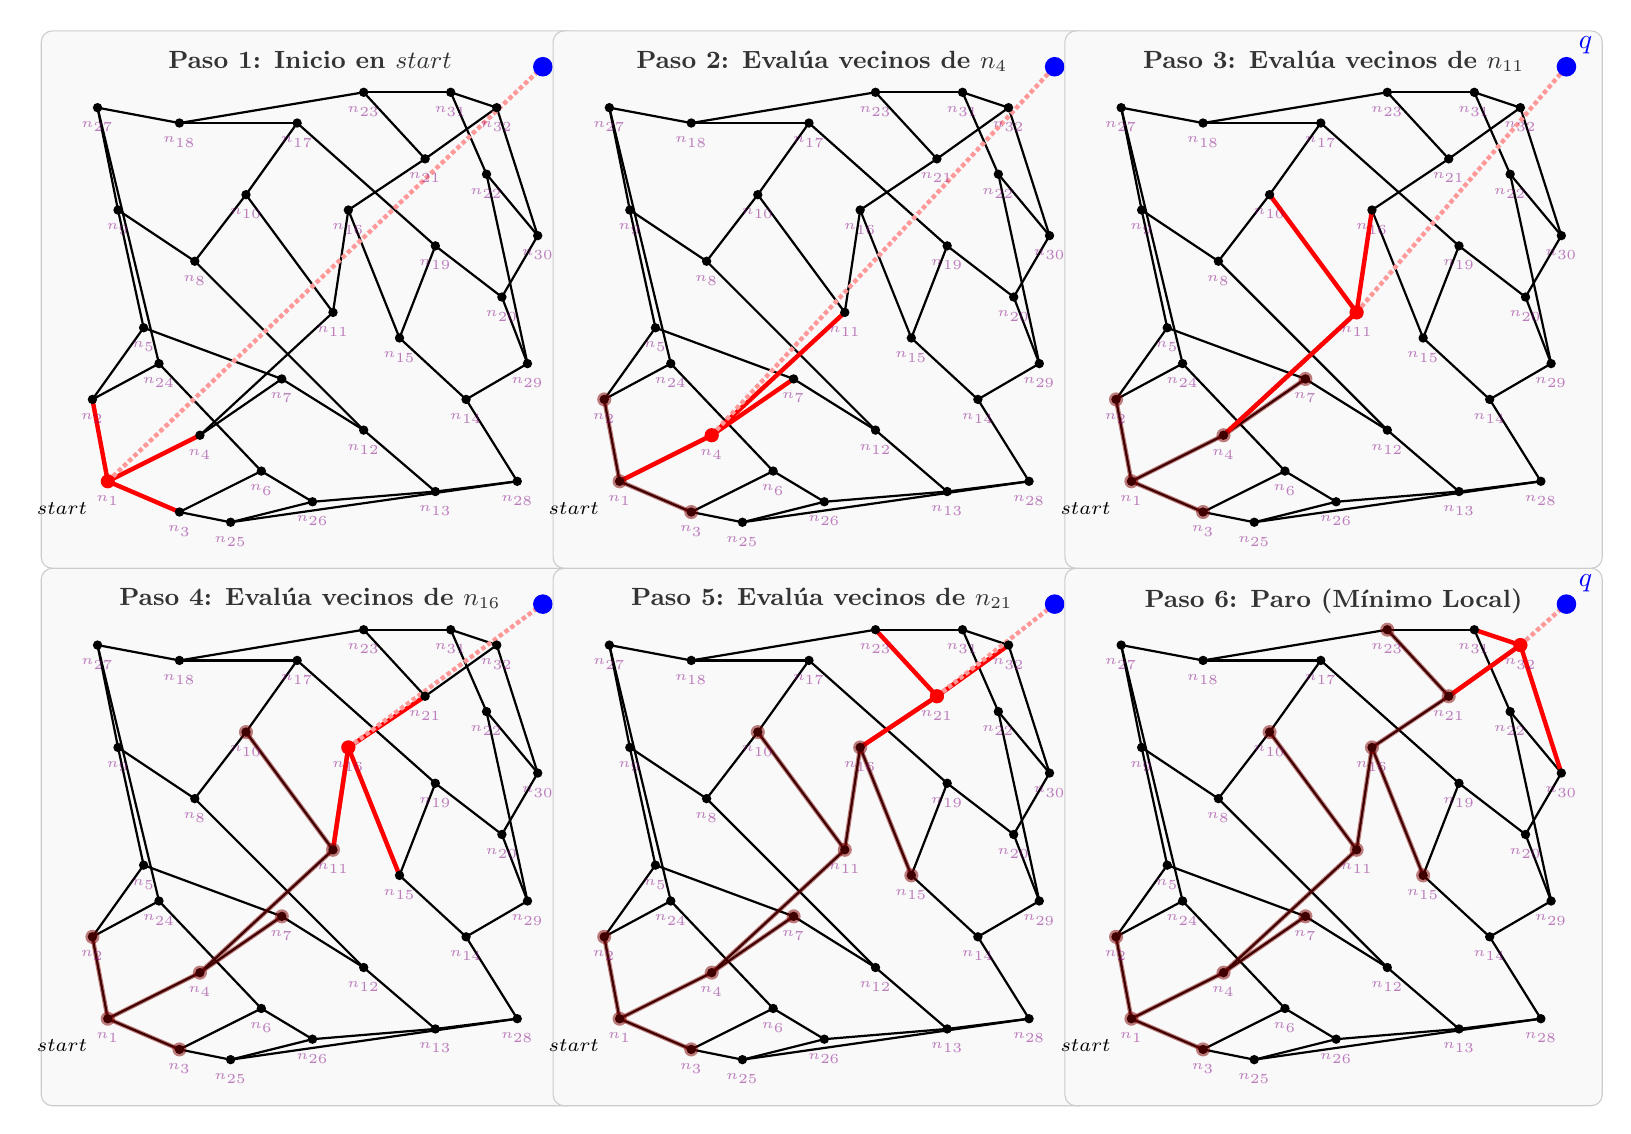
\begin{tikzpicture}[
    scale=0.65, 
    % Estilos de nodos
    base node/.style={circle, fill=black, inner sep=1.2pt},
    query node/.style={circle, fill=blue, inner sep=2.5pt},
    active node/.style={circle, fill=red, inner sep=1.8pt},
    trace node/.style={circle, fill=red!50!black, inner sep=1.8pt, opacity=0.5}, % Halo oscuro opaco al 0.5
    node label/.style={below=1.5pt, font=\tiny, text=violet, opacity=0.5}, % Etiquetas violetas opacas al 0.5
    % Estilos de aristas
    base edge/.style={thick, black},
    active edge/.style={ultra thick, red},
    trace edge/.style={ultra thick, red!50!black, opacity=0.5}, % Traza oscura opaca al 0.5
    eval line/.style={densely dotted, ultra thick, red!40}
]

% Bucle para generar la cuadrícula de 6 pasos (2 filas x 3 columnas)
\foreach \step/\xshift/\yshift/\act/\nI/\nII/\nIII/\title in {
    1/0/10.5/c1/c2/c3/c4/{Paso 1: Inicio en $start$},
    2/10.0/10.5/c4/c1/c7/c11/{Paso 2: Evalúa vecinos de $n_4$},
    3/20.0/10.5/c11/c4/c10/c16/{Paso 3: Evalúa vecinos de $n_{11}$},
    4/0/0/c16/c11/c15/c21/{Paso 4: Evalúa vecinos de $n_{16}$},
    5/10.0/0/c21/c16/c23/c32/{Paso 5: Evalúa vecinos de $n_{21}$},
    6/20.0/0/c32/c21/c30/c31/{Paso 6: Paro (Mínimo Local)}
}{
    \begin{scope}[shift={(\xshift, \yshift)}]
        
        \defineCoordinates
        
        % Caja y Título
        \draw[draw=black!20, fill=gray!5, rounded corners] (-0.5, -0.5) rectangle (10.0, 10.0);
        \node[font=\small\bfseries, color=black!80, anchor=north] at (4.75, 9.8) {\title};

        % 1. Capa de fondo: Grafo base
        \drawBaseEdges
        
        % 2. Capa media: Traza histórica (Halo oscuro, opacity=0.5)
        \drawHistoryEdges{\step}
        
        % 3. Capa superior: Aristas del paso activo (Rojo brillante)
        \draw[active edge] (\act)--(\nI);
        \draw[active edge] (\act)--(\nII);
        \draw[active edge] (\act)--(\nIII);
        
        % 4. Línea de evaluación
        \draw[eval line] (\act) -- (q);

        % 5. Capa de Nodos base y Etiquetas Violetas
        \foreach \i in {1,...,32} { 
            \node[base node] at (c\i) {}; 
            \node[node label] at (c\i) {$n_{\i}$}; 
        }
        
        % 6. Capa de Nodos históricos (opacity=0.5)
        \drawHistoryNodes{\step}

        % 7. Nodos especiales
        \node[below left=4pt, font=\scriptsize\bfseries, black] at (c1) {$start$}; % Ajustado para no sobreponer la etiqueta n1
        
        \node[query node] at (q) {};
        \node[above right=1pt, font=\bfseries, blue] at (q) {$q$};
        
        \node[active node] at (\act) {};

    \end{scope}
}

\end{tikzpicture}
\end{document}
